\documentclass{article}
\usepackage[utf8]{inputenc}
\usepackage{url}
\usepackage{ctex}
\usepackage{geometry}
\usepackage{fancyhdr}
\usepackage{lastpage}
\usepackage{subfigure}
\usepackage[graphicx]{realboxes}
\usepackage{color}
\usepackage{hyperref}
\usepackage{titlesec}

\geometry{a4paper, margin=1in}

\pagestyle{fancy}
\fancyhf{}
\fancyhead[L]{iFuProcessor设计报告}
\fancyhead[R]{\today}
\fancyfoot[C]{\thepage\ / \pageref{LastPage}}

\begin{document}

\pagestyle{plain}

\begin{center}
    \Huge{iFuProcessor设计报告}
\end{center}

\vspace{30mm}

\begin{figure}[h]
    \centering
    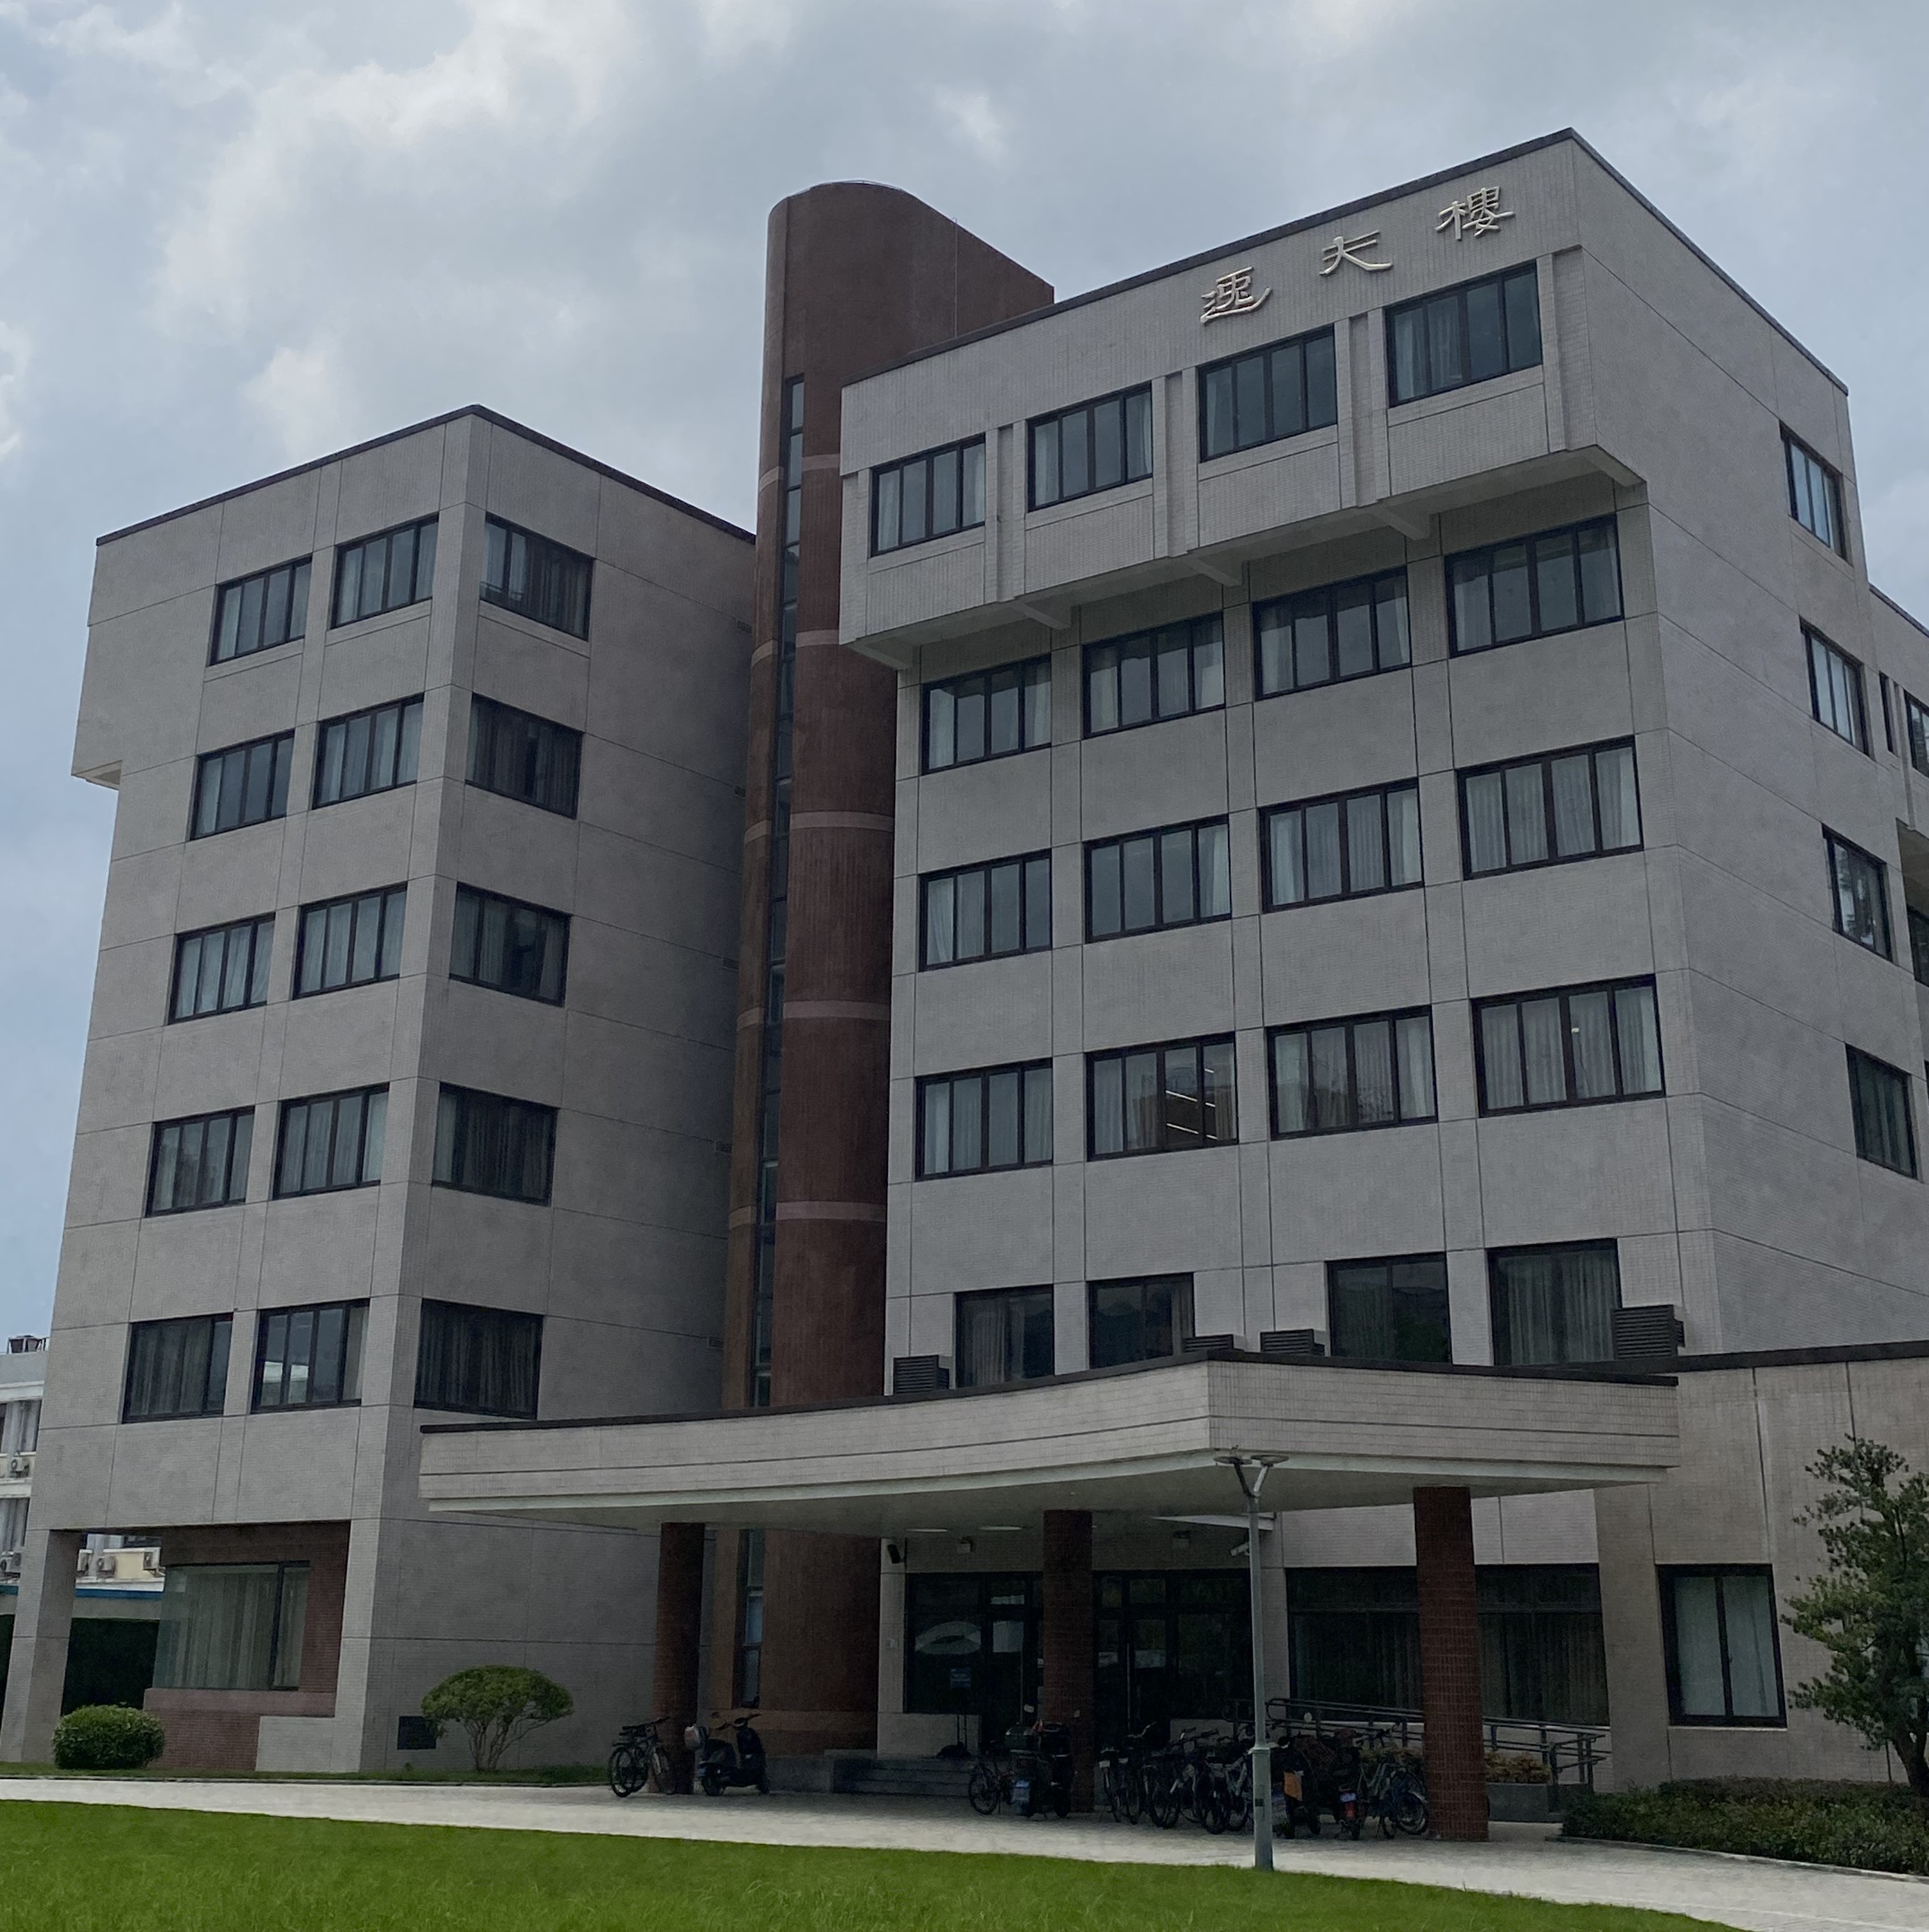
\includegraphics[width=0.8\linewidth]{./imgs/if.jpg}
\end{figure}
\vfill

\begin{center}
    \Large{肖德\ 刘思远\ 李丛林\ 章云天}
    
    \large{指导教师:张亮\ 张为华}

    \normalsize{\today}
\end{center}

\newpage
\pagestyle{fancy}

\setcounter{tocdepth}{3}
\tableofcontents

\section{项目概述}
\subsection{项目背景}
本项目是第八届“龙芯杯”全国大学生计算机系统能力培养大赛(NSCSCC 2024)的参赛作品。\par
项目实现了一款基于龙芯架构32位精简版(LoongArch32-Reduced,LA32R)指令集的乱序多发射CPU——iFuCore,并为之构建了一款SoC——iFuSoC。iFuCore能够在龙芯实验箱上通过全部功能测试、性能测试。借助iFuSoC,iFuCore能够通过uboot加载运行Linux操作系统,并且支持完善的外设驱动。\par
本项目已于Github上开源。\url{https://github.com/iFuProcessor}

\subsection{开发语言}
本项目使用Chisel编写。借助Chisel的高层抽象,可以更加方便地实现复杂的硬件逻辑,同时也支持更加灵活的参数化设计。\par
在本项目的设计和开发中,主要参考了The Berkeley Out-of-Order Machine (BOOM)的设计模式和组织方式。\par

\section{微架构设计}
\subsection{整体架构}
iFuCore是乱序三发射结构设计,目前支持LA32R除CACOP、浮点外的全部指令(在当前的实现中,CACOP被实现为IBAR指令,未实现对Cache的精细操作)。\par
借助指令缓冲(Fetch Buffer),iFuCore实现了前后端解耦。前端包括分支预测、取指令、预译码;后端包括译码、重命名、派遣、发射、读寄存器、执行、写回,此外,重排序缓冲(Reorder Buffer,ROB)在指令写回后,会进行异步提交。\par
访存子系统中,iFuCore实现了访存执行单元(Load/Store Unit,LSU),其中包含了Load/Store Queue、两条访存流水线。借助LSU,iFuCore实现了Load/Store指令的乱序执行,并保证其内存序的正确性。相应的,iFuCore配备了访存宽度为2的非阻塞数据缓存(Nonblocking DCache)。\par
\begin{figure}[h]
    \centering
    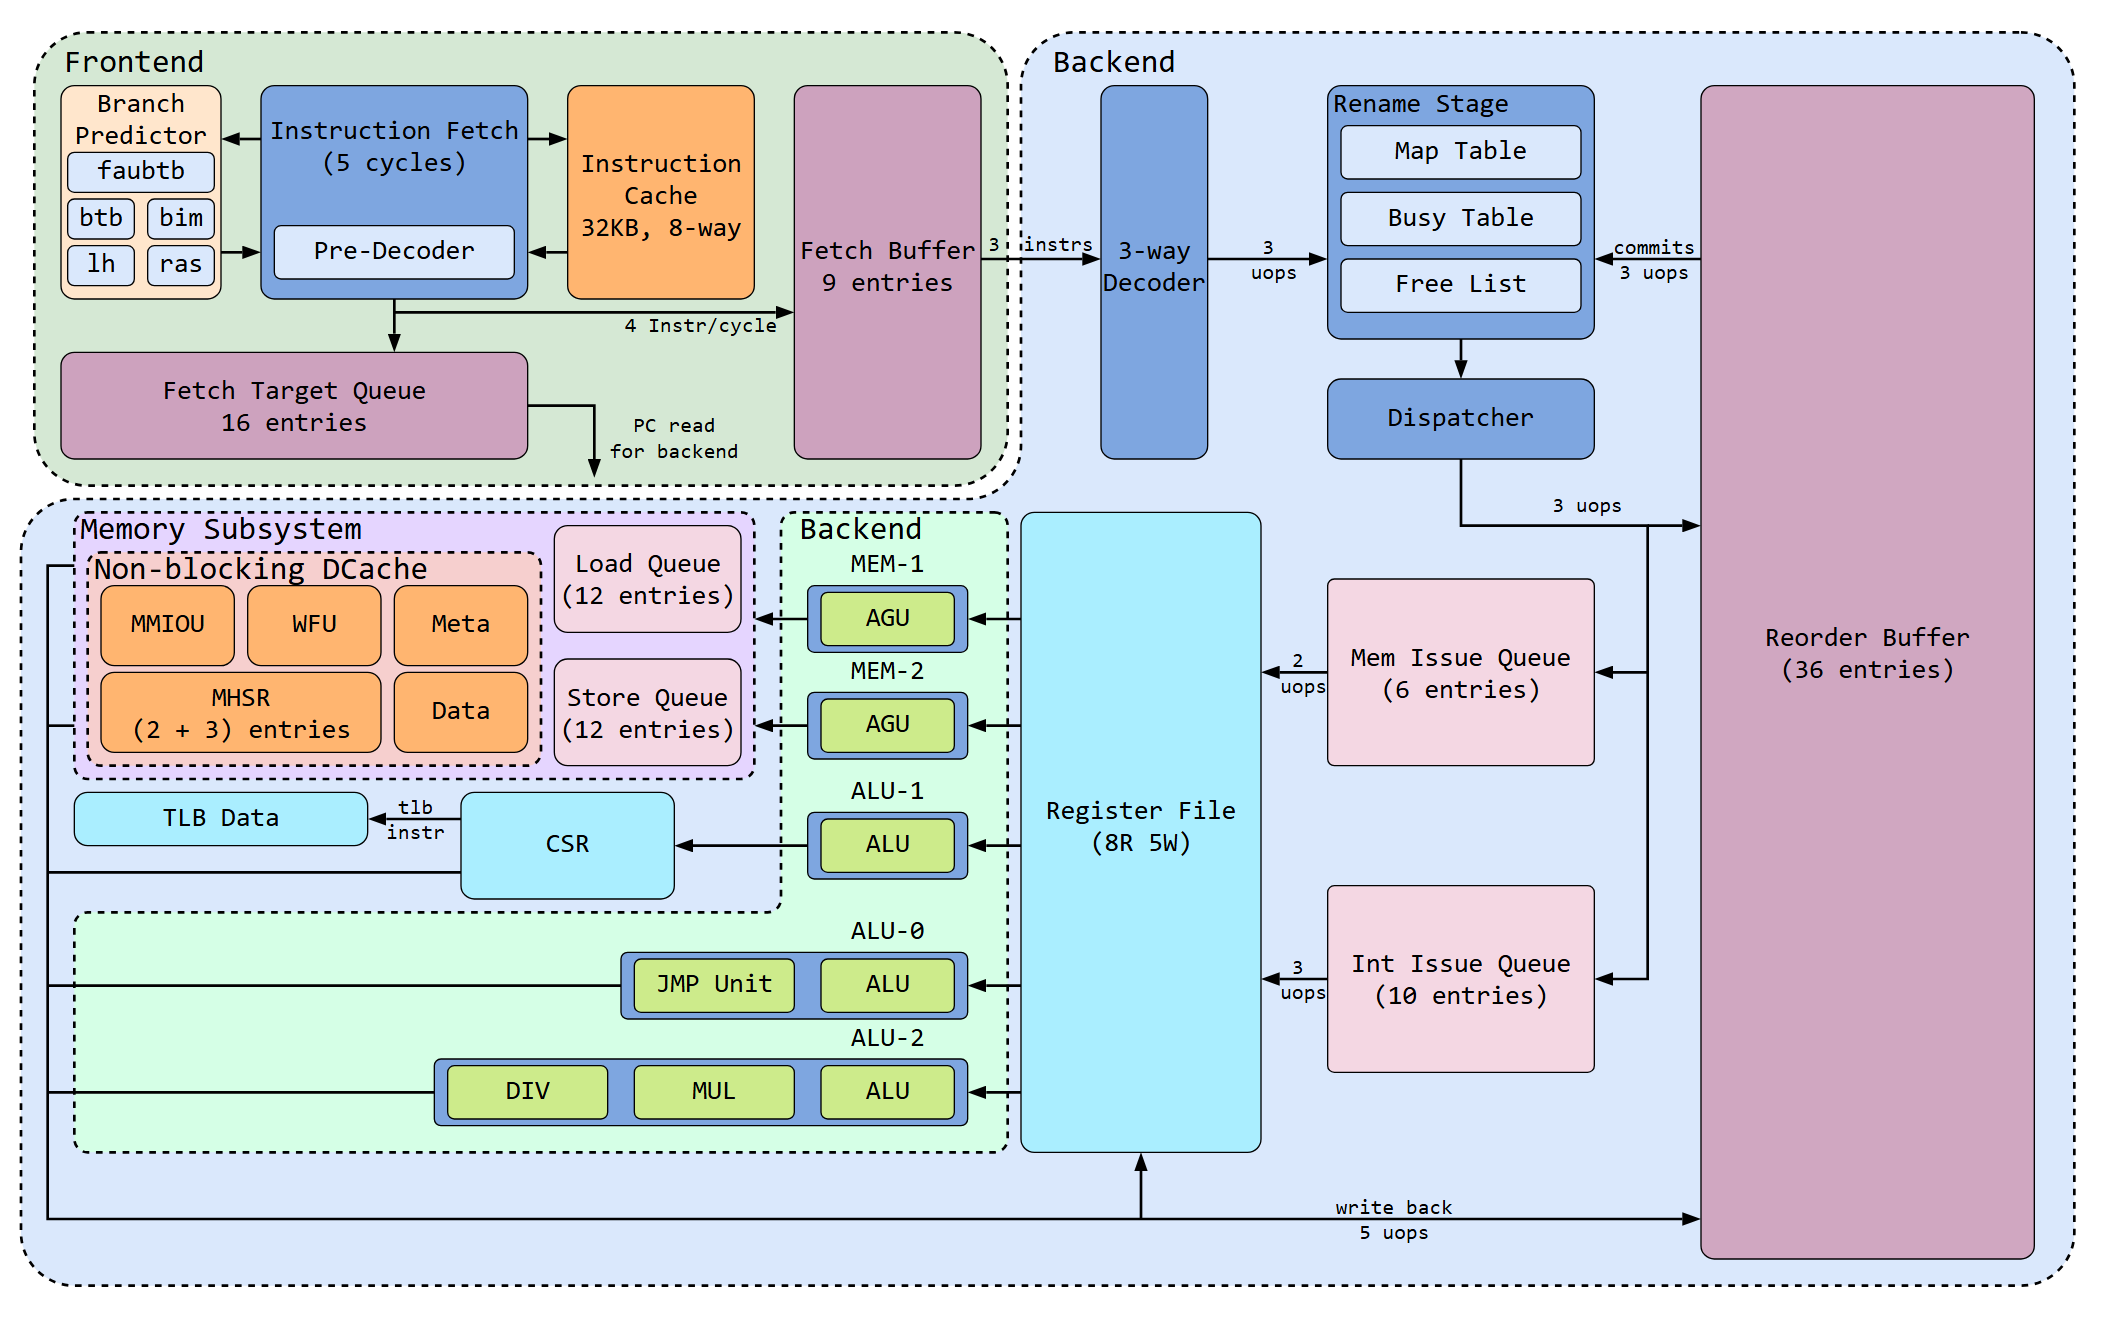
\includegraphics[width=\linewidth]{./imgs/Core.png}
    \caption{整体架构}
\end{figure}

\subsection{前端}
前端流水线共五级(下称S0-S4),分支预测和取指令同时进行。在默认配置下,前端每周期可以取出对齐的4条指令,送入指令缓冲(Fetch Buffer)。同时将预测和取指过程产生的信息送入取指目标队列(Fetch Target Queue,FTQ),供重定向与分支预测器(Branch Predictor, BPD)更新使用。\par
\subsubsection{分支预测器(Branch Predictor, BPD)}
分支预测采用多级混合预测的架构,主要包括全相联分支目标缓存(Full-associave Micro Branch Target Buffer, FaUBTB)、2位饱和计数器表(Bi-Model Table, BIM)、分支目标缓存(Branch Target Buffer, BTB)、局部历史(Local History, LH)组成。\par
BPD在S0-S3阶段运行。对于S0送入的每个(按4条指令对齐的)PC,BPD在S1-S3对4条指令中的每条输出预测的结果(跳转/不跳转与目标地址)。\par
BPD的更新在指令提交后,由FTQ将信号送入并更新。\par
\paragraph{全相联分支目标缓存(Full-associave Micro Branch Target Buffer, FaUBTB)}
FaUBTB在S1运行,用于及时提供一个无气泡的预测。FaUBTB包含4个全相联的表项,每个表项包含跳转目标地址、2位饱和计数器、是否条件跳转指令、tag。\par
\paragraph{2位饱和计数器表(Bi-Model Table, BIM)}
BIM在S0-S2运行。用PC的高位索引大小为512的2位饱和计数器表,根据表项预测是否跳转。\par
\paragraph{分支目标缓存(Branch Target Buffer, BTB)}
BTB在S0-S2运行。BTB表为2路64组相联结构。每个BTB项包含跳转目标地址、是否条件跳转指令。另外对每个项保存PC的高位,用于判断是否命中。\par
\paragraph{局部历史(Local History, LH)}
LH在S0-S3运行。用PC的高位索引一个64项的局部历史表,再用该PC的局部历史索引一个8192项的2位饱和计数器表。根据饱和计数器的值预测是否跳转。\par

\subsubsection{取指令}
取指令包括地址翻译、指令缓存(ICache)。\par
\paragraph{指令缓存(ICache)}
ICache为VIPT的8路64组相联结构,每个cache行包含16条指令,总大小32KB。替换策略采取LRU。由于AXI总线的数据宽度为32,利用AXI的突发传输机制,传输16拍32位数据,并在ICache内部重填,以此在一次总线事务中重填一个cache行。\par
\subsubsection{预译码(PreDecode)}
PreDecode在S2阶段,将ICache返回的指令译为以下信号:1.是否分支指令;2.是否条件跳转指令;3.是否call指令(将PC+4写入\$r1的分支指令);4.是否return指令(跳转到\$r1的指令);5.跳转目标地址。这些信息一方面在S3结合RAS进一步更正分支预测的结果,另一方面存入FTQ,用于提交时更新分支预测器。
\subsubsection{返回地址栈(Return Address Stack, RAS)}
RAS在S3阶段,包含8个项,存放预译码得到的call指令的下一个PC,用于预测return指令的目标地址。
\subsubsection{指令缓存(Fetch Buffer)}
Fetch Buffer是前端与后端的分界点。Fetch Buffer最多存放9条指令,在S4接收前端取到的指令,压缩存入,并以每周期三条的速度发送到后端执行。
\subsubsection{取指目标队列(Fetch Target Queue, FTQ)}
FTQ主要存储BPD与RAS在预测过程中提供的信息,用于在指令提交时更新BPD以及在发生重定向时部分重置RAS。

\subsection{后端}
处理器的流水线后端负责指令的重命名与乱序执行。在默认配置下,后端每周期可以从Fetch Buffer中取出3条指令并执行。取出的指令经译码、重命名后,依据其指令类型,被派遣到访存发射队列(Memory Issue Queue,MIQ)或整数发射队列(Int Issue Queue,IIQ)中。MIQ每周期可以选出至多2条指令发射到2个完全对称的地址生成单元(Address Generation Unit,AGU)中,由AGU向LSU发送访存请求,并接收访存结果;IIQ每周期可以选出至多3条指令发射到3个不完全对称的整数单元(后文中也称ALU)中执行。指令经执行后,将结果写回寄存器堆(Register File)并通知ROB,由ROB顺序提交。\par

\subsubsection{译码}
指令译码阶段负责将Fetch Buffer中的指令解码为微码(Micro Op,$\mu$op),交由后端流水线执行。\par
对于译码器及控制信号,参考了BOOM的设计,将译码分为译码逻辑(DecodeLogic)和译码表(DecodeTable)两部分,以便于后续的扩展和维护。\par

\subsubsection{重命名}
iFuCore采用显式重命名,在重命名阶段管理和维护逻辑寄存器与物理寄存器之间的映射,通过对逻辑寄存器重命名,消除指令间的依赖以完成乱序调度。在本阶段中,主要涉及到三个模块:BusyTable、FreeList和MapTable。\par

\paragraph{BusyTable}
BusyTable用于记录每一个物理寄存器的状态,指示其是否就绪。指令可以从中获取到其操作数是否就绪。

\paragraph{FreeList}
FreeList记录当前空闲的物理寄存器。对于需要写回的指令,从中选取一个物理寄存器进行分配。

\paragraph{MapTable}
MapTable记录逻辑寄存器到物理寄存器的映射关系。指令从中读取操作数对应的物理寄存器号,并修改其目的操作数的映射关系。

\subsubsection{派遣}
在此阶段,指令依据其类型被派遣到MIQ或IIQ中。若其对应的发射队列已满,则在此进行阻塞,直至其能够进入对应的发射队列。同时,被派遣的指令还会送入ROB中,以便后续的提交。\par
派遣是处理器顺序执行和乱序执行的分界点,在此之前,指令均以对齐的方式顺序执行;在此之后,指令在IQ中乱序调度并执行。\par

\subsubsection{发射}
iFuCore采用混合式发射队列,依据不同的指令类型,分为MIQ和IIQ,其中维护所有尚未执行的指令,将之置于一个发射槽(Issue Slot)中。为了优化发射效率,iFuCore采用压缩队列的设计,每周期每条指令至多向前移动3个发射槽,在选择时,优先选择前方的发射槽即可。\par
IQ会监听各个功能单元的唤醒信号,并将其传递给每一个Issue Slot。由于采用发射后读寄存器的方式,此处只需广播物理寄存器号,避免广播数据带来的开销。\par

\subsubsection{读寄存器}
被发射的指令在此阶段从寄存器堆中读取操作数,同时也会进行旁路转发。

\subsubsection{执行}
iFuCore的执行单元分为两大类:访存单元和整数单元。\par
访存单元共计2个,访存指令会在此阶段计算访存地址,对于Store类指令,此阶段还需负责传递数据。在完成计算后,会将访存请求发送给LSU,交由LSU进一步进行乱序执行。同时,LSU会返回此前发送的访存请求的结果,访存单元负责将其写回。\par
整数单元共计3个,不完全对称。每个整数单元都能够执行普通的算术指令和分支指令。对于需要使用PC的指令,因为$\mu$op中不含PC,需要向FTQ请求,因此第一个整数单元额外配置了与FTQ交互的接口,执行此类指令。第二个整数单元额外负责执行CSR指令及RDCNT指令。第三个整数单元额外负责执行乘除法指令。\par
出于时序考虑,乘法器利用DSP48E1实现。除法器参考香山处理器的设计,实现了SRT16除法器。\par

\subsubsection{写回}
此阶段收集所有功能单元的执行结果,对于需要写回的指令,将其结果写回寄存器堆。同时,会通知ROB该指令已经执行完毕,可以提交。\par
对于CSR指令,会在此阶段将指令及其操作数传递给CSR模块,进行CSR的读写操作。\par

\subsubsection{指令提交}
ROB会维护所有尚未提交的指令,并将其按序提交。在默认配置下,ROB每周期可以对齐的提交至多3条指令。当中断或异常发生时,ROB会通过回滚来恢复处理器状态,并且通知其余模块进行相应的处理。\par
对于部分特殊指令,参考BOOM的设计,引入unique机制,限制处理器的乱序执行,以保证指令的正确性。\par
关于ROB的组织形式,参考BOOM的设计,分为多个Bank组织,虽然会因为指令对齐带来一定程度的空间浪费,但是可以减少ROB每列的读写口数目,简化逻辑,提高频率。\par


\subsection{访存子系统}
访存子系统包括LSU、NonBlocking DCache等模块。其中,LSU是暴露给外部的访存执行单元,是CPU后端架构和访存子系统的接口模块,负责协调访存的乱序执行、地址翻译、异常检测,以及将访存$\mu$op转化为DCache的请求。非阻塞数据缓存是访存子系统的核心模块,负责处理访存请求,通过总线与内存交互。\par
访存子系统保证store指令之间严格顺序执行,load指令乱序执行,load指令与store指令之间乱序执行,但是保证访存的内存序正确。\par
访存子系统拥有两条访存执行流水线,可以同时执行至多两个访存请求,增加了访存请求的吞吐量。非阻塞数据缓存,尽可能提高乱序执行能力,减少阻塞。\par
本项目尽最大可能提高核的访存能力,在当前访存架构设计下,对于部分访存压力较大的测试点性能提升明显。
\subsubsection{访存执行单元(Load/Store Unit,LSU)}
总体来看,LSU共有4个流水级(下称S0-S3)。iFucore为地址翻译以及地址相关异常检测设计了一个独享的周期(S0),以减轻时序负担。\par
S1周期进行相关异常信息的汇总处理,进行内部资源调度,接收流水线中传入的访存$\mu$op,以及后续传来的数据,物理地址等信息,存储在Load Queue、Store Queue中,并且选择出一个或一对访存请求发送给DCache。\par
S2周期进行转发判断。新load请求在传入地址后,从Store Queue中进行地址的匹配判断。新的store请求在传入地址后,会对目前所有Load Queue中进行地址的匹配判断,检查访存违例现象,保证访存的顺序。同时进行推测唤醒,根据issue单元传来的推测唤醒信号,将对应load唤醒执行。\par
S3根据前一周期的判断,确定访存违例的load指令。如果上周期有出现异常或被转发完成的load请求,就会发送S1-S3周期维护内部状态,根据新完成的指令调整内部访存队列,将可能的异常信息报告给ROB。\par
\subsubsection{非阻塞数据缓存(NonBlocking DCache)}
DCache包括3级流水。S1发起读meta请求,S2结合meta返回的hit信息,发起读data请求,S3根据读出的数据,进行读取数据或写入数据的操作。\par
DCache为4路64组相联,每行64B(AXI一次最大的传输请求数),使用PIPT匹配模式。DCache内部组件包括Meta、Data。Meta维护地址的匹配,Data维护缓存行数据。\par
DCache内部的WFU(Write-Fetch-Unit)用于进行缓存行的写回和回填操作,一个完整的写回/回填操作流程会处理一个cache行。从具体执行层面,是以单个字为单位进行的,即每个周期处理一个字的数据。向内存进行数据行写回的时候,会将cache行的数据写回到内存,连续16个周期读取单个字,存入WFU内部的buffer中,然后由WFU进行写回。向cache行进行回填的时候,由于AXI存在随机延迟,在回填16个字的过程中存在若干“空隙”周期,为充分实现非阻塞,每当axi有rvalid,s0就将该周期任务设置成重填行,在随机延迟的等待时间里,可以正常处理其他请求。\par
DCache实现了MSHR(Missing Status Handling Register)进行miss的处理,miss请求会存入MSHR,分为一二级表项,以行地址为单位组织成并查集格式。一级表项用于表示待取地址,二级表项则是具体的请求项,依赖某一个一级表项。MSHR中共有2个一级表项,3个二级表项。当一个地址所需的cache行被WFU取好之后,会来到MSHR里面清除对应的一级表项,唤醒二级表项中的请求,以发起后续重发请求。由于存在两条流水线,可能同时发生miss,因此向MSHR写入需要进行一次仲裁,选择一条流水线中的请求进行写入。\par
DCache通过MMIOU(Memory Mapped IO Unit)实现至多单个字的uncache请求,一次最多接收一个uncache请求。在执行uncache请求的过程中,不允许其他uncache请求执行,来保证uncache请求的顺序性。MMIOU直到执行完毕,才会占用流水线以返回uncache请求的结果。\par
DCache中各个流水段存在一个状态信息,标识当前流水段正在执行的任务种类,目前的架构实现中,DCache共有11个状态:\par
\begin{itemize}
    \item s\_replay: 重发此前miss的请求,从MSHR发出
    \item s\_wb: 将cache行写回到内存,此处WFU发出读cache行字的请求
    \item s\_refill: cache行回填。此处WFU发出写cache行字的请求
    \item s\_replace\_find: 替换行查找。发生miss时并不当即寻找miss行,而是在MSHR发出请求的时候确定替换的位置,将该请求传递给WFU
    \item s\_lsu: LSU发起的普通的访存请求,最多一次接收两个请求执行
    \item s\_mmio\_req: LSU发起的uncache请求,送给MMIOU执行
    \item s\_mmio\_resp: MMIOU执行完毕的请求,返回给LSU
    \item s\_fence\_read: 清空cache行的过程中,取出一个cache行的数据
    \item s\_fence\_clear: 写回一个脏行之后,清空对应的Meta信息
    \item s\_cacop: 执行CACOP指令
    \item s\_nil: 标记该流水段为空闲
\end{itemize}

\subsection{TLB}
出于时序考虑,iFuCore参考了MaRiver的设计,将TLB实现为对体系结构隐藏的两级结构,其中包括L0-iTLB、L0-dTLB、L1-TLB。\par
出于简化设计的考虑,当L1-TLB被修改时,会将L0-iTLB、L0-dTLB全部清空以维护一致性。在L0-iTLB和L0-dTLB中,均实现了直接地址翻译模式和映射地址翻译模式(包括直接映射模式与页表映射模式)。\par
\subsubsection{L0-TLB}
在L0-TLB的项中,除了表项本身,还包括一个exist位,用于标记表项是否存在于L1-TLB中。当一个地址未命中L0-TLB,不会立即抛出TLBR异常,而是抛出一个架构不可见的异常L0TLB\_MISS,同时向L1-TLB发起查询。如果查询到,则将表项填入到L0-TLB,否则,构造一个exist位为0的项,填入L0-TLB。一个地址若命中了一个exist位为0的项,则抛出TLBR异常。\par
\subsubsection{L1-TLB}
L1-TLB并不负责地址翻译,而是维护架构要求的32个TLB表项。TLB指令直接操作L1-TLB。每当L1-TLB发生修改,都会将L0-TLB中的所有表项清空,以保证一致性。\par
L1-TLB对L0-TLB暴露为1读口。当L0-TLB发生miss时,会进行仲裁,选择一方来进行查询。\par

\subsection{数据总线}
处理器对外暴露一条AXI3总线,用于与内存及外设通信。处理器内共计3处需要与总线交互:ICache、WFU、MMIOU。\par
为了简化设计,iFuCore采用核内SMA(Simple Memory Access)总线,以支持上述3处与总线的交互。\par
鉴于访存模式的相似性,SMA总线支持访存请求的代理。上层模块只需传递少量必要信息,而且拥有独占总线的抽象接口。在SMA总线内部,使用仲裁器来处理多个请求的冲突,并且实现基于事务ID的乱序访存。最终,SMA总线会将访存请求转发至AXI3总线。\par

\subsection{微架构优化}
\paragraph{多级分支预测器}
BPD在S1-S3每周期输出一次预测结果,在前端发现更晚的预测与更早的预测不符时,在前端内部重定向,采用更晚的预测。这使得BPD能够加入更复杂的多周期预测器;同时对于更容易预测的指令,能够在较早的周期通过更简单的预测器得到正确的预测结果。\par
\paragraph{分支标签(Branch Tag)}
为每条指令赋予一个Branch Tag,跨分支指令时Branch Tag改变。这样能在分支指令完成执行时,如果发现分支预测错误,将核内在该分支指令之后的指令全部消除。这样能够在发现分支预测错误时及时通知前端开始重新取指,而无需等到分支指令提交后再进行重定向。iFuCore支持8个Branch Tag,即允许最多8条分支指令在后端流水线中。\par
\paragraph{FTQ存放PC}
部分指令在执行过程中需要使用这条指令的PC。采用将PC存放在FTQ中的设计,需要使用PC的指令在执行时向FTQ请求。这样能避免在$\mu$op中存放32位的PC,且一次取指的4条指令能共用一个PC。\par
\paragraph{快速唤醒} 
为了实现连续发射,iFuCore采用了快速唤醒的设计,即在指令发射时,若其结果可被转发,则直接唤醒其后继指令。\par
\paragraph{访存推测唤醒} 
为了优化load-use延迟,iFuCore引入了访存推测唤醒机制,当Load指令被LSU选中发送到DCache时,会唤醒其后继指令,若后续发生DCache Miss,则会取消唤醒。\par
\paragraph{发射掩码} 
经测试,并非每个Issue Slot中的指令都能发射,为了降低选择电路的规模,iFuCore引入了发射掩码,只有掩码为1的指令才能发射。在实现中,将IIQ中30组请求(共计10项Issue Slot,3个整数单元)降低至21组,在保持IPC几乎不变的情况下,有效简化了发射逻辑。\par
\paragraph{store类指令拆分} 
鉴于Store类指令需要2个操作数,且二者往往不能够同时就绪,iFuCore将Store类指令拆分为STA和STD两个$\mu$op。经此设计,Store类指令的发射更加灵活,其需要的操作数也减少至1个。在此基础上,减少访存单元的寄存器读端口数目,由于总计发射宽度为5,将读口数从10减少至8,能够有效降低资源的使用。\par
\paragraph{SMA总线乱序访存} 
经测试,相较于简单的总线仲裁器,SMA总线提供的乱序访存机制能够有效降低总线交互代码的复杂度,并且能够有效提高访存性能,在提供的性能测试点中,SMA总线能够带来约$0.5\% \sim 5\%$的IPC提升。\par

\subsection{性能测试Benchmark}
表1给出了iFuCore(80MHz)在大赛性能测试perf\_test中的20个Benchmark中相对参考核openla500(40MHz)的加速比。结果使用的性能计数器读数为连续三次运行的最小值。
\begin{table}[h]
    \begin{center}
        \begin{tabular}{|cc|cc|}
            \hline
            Benchmark & IPCUp & Benchmark & IPCUp \\
            \hline
            bitcnt &  1.99       & fireeye A0 & 1.96\\
            bubble sort & \textcolor{blue}{1.34}   & fireeye B2 & 2.04\\
            coremark & 1.71      & fireeye C0 & \textcolor{blue}{1.10}\\
            crc32 & \textcolor{red}{2.86}        & fireeye D1 & \textcolor{red}{2.50}\\
            dhrystone & 2.00     & fireeye I2 & 2.06\\
            quick sort & \textcolor{blue}{1.37}    & inner product & 2.05\\
            select sort & 2.10   & lookup table & \textcolor{red}{2.35}\\
            sha & \textcolor{red}{2.57}          & loop induction & 2.15\\
            stream copy & 1.97   & my memcmp & \textcolor{red}{3.10}\\
            string search & 1.67 & minimax sequence & 2.09\\
            \hline
            Geo.Mean & 1.990 & - & - \\
            \hline
        \end{tabular}
        \caption{测试结果}
    \end{center}
\end{table}

\section{SoC设计}
iFuCore通过iFuSoC驱动外设。iFuSoC包含了以下外设:\par
\begin{itemize}
    \item DDR3 DRAM(K4B1G1646G)
    \item NAND Flash(K9F1G08U0C)
    \item SPI Flash(EN25F80)
    \item UART 串口控制器
    \item Ethernet 控制器(DM9161AEP)
    \item GPIO
    \item LCD 显示器(NT35510)
    \item VGA 输出设备
    \item PS2 输入设备
\end{itemize}
\begin{figure}[h]
    \centering
    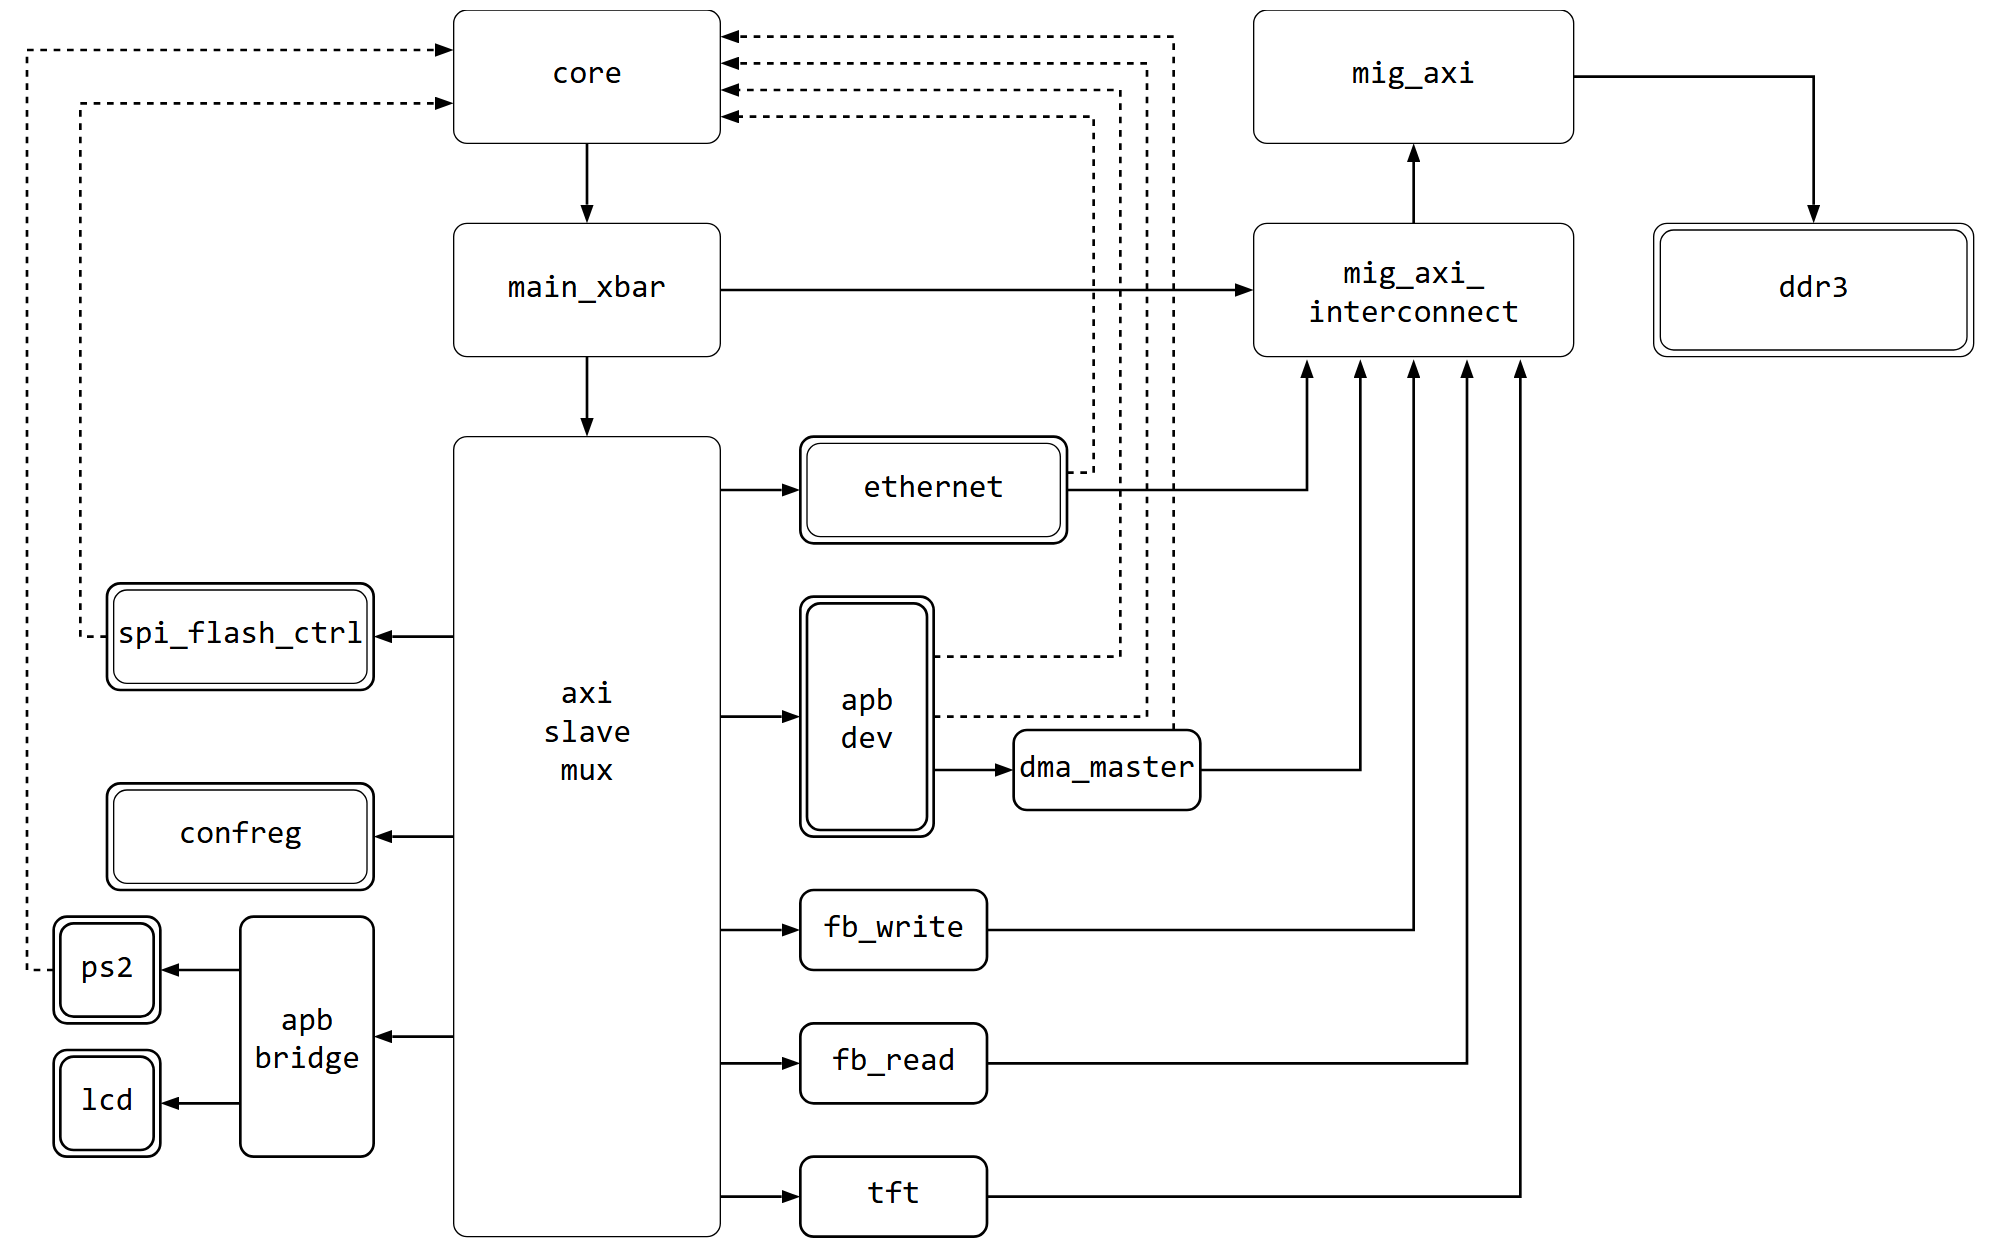
\includegraphics[width=0.5\linewidth]{./imgs/SoC.png}
    \caption{iFuSoC 结构图}
\end{figure}

\subsection{地址分配}
SoC 对各外设的地址映射规则如表2所示。\par
\begin{table}[h]
    \begin{center}
        \begin{tabular}{|c|c|c|c|}
            \hline
            地址段                              & 起始地址    & 结束地址    & 分配大小\\
            \hline
            DDR3 Memory                         & 0x00000000 & 0x07FFFFFF & 128 MB\\
            SPI Memory                          & 0x1C000000 & 0x1C0FFFFF & 1MB\\
            TFT Controller                      & 0x1D010000 & 0x1D01FFFF & 64 KB\\
            PS2 Controller                      & 0x1D020000 & 0x1D02FFFF & 64 KB\\
            NT35510 Controller                  & 0x1D030000 & 0x1D03FFFF & 64 KB\\
            Video Frame Buffer Read Controller  & 0x1D050000 & 0x1D05FFFF & 64 KB\\
            Video Frame Buffer Write Controller & 0x1D060000 & 0x1D06FFFF & 64 KB\\
            Configuration Registers             & 0x1FD00000 & 0x1FD0FFFF & 64 KB\\
            UART Controller                     & 0x1FE00000 & 0x1FE0FFFF & 64 KB\\
            NAND Controller                     & 0x1FE70000 & 0x1FE7FFFF & 64 KB\\
            SPI Controller                      & 0x1FE80000 & 0x1FE8FFFF & 64 KB\\
            Ethernet Controller                 & 0x1FF00000 & 0x1FF0FFFF & 64 KB\\
            \hline
        \end{tabular}
        \caption{iFuSoC 地址映射表}
    \end{center}
\end{table}

\subsection{外设控制器}
iFuSoC移植了一些已有的外设控制器,详见表3。iFuSoC沿用并拓展了chiplab使用的外设中断号分配如下表。\par
\begin{table}[h]
    \begin{center}
        \begin{tabular}{|c|c|c|}
            \hline
            外设 & 控制器来源 & 中断位 \\
            \hline
            Ethernet    & Chiplab                 & HWI0 \\
            UART        & Chiplab                 & HWI1 \\
            SPI Flash   & Chiplab                 & HWI2 \\
            NAND Flash  & Chiplab                 & HWI3 \\
            DMA         & Chiplab                 & HWI4 \\
            PS2         & Altera                  & HWI5 \\
            VGA TFT     &  Xilinx                 & -    \\
            Video Framebuffer Read/Write &  Xilinx  &  - \\
            LCD         & NOP-Processor           & -    \\
            \hline
        \end{tabular}
        \caption{iFuSoC 控制器配置}
    \end{center}
\end{table}

\section{系统软件}
在功能测试与性能测试的基础上,使用uboot和Linux来验证CPU实现的正确性。
\subsection{uboot}
本项目使用uboot作为Linux的引导程序。使用到的uboot修改自龙芯仓库的la32r-uboot。实现了自定义开机启动欢迎界面与开发板GPIO的初始化驱动。\par
\begin{figure}[h]
    \centering
    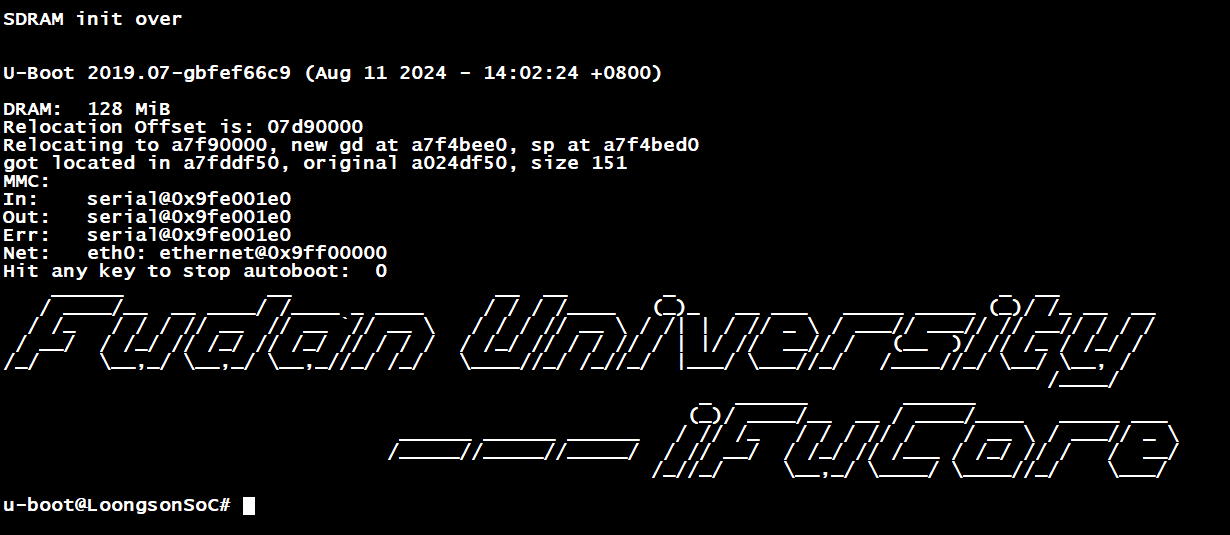
\includegraphics[width=0.5\linewidth]{./imgs/uboot_hello.png}
    \caption{开机启动界面}
\end{figure}
\begin{figure}[h]
    \centering
    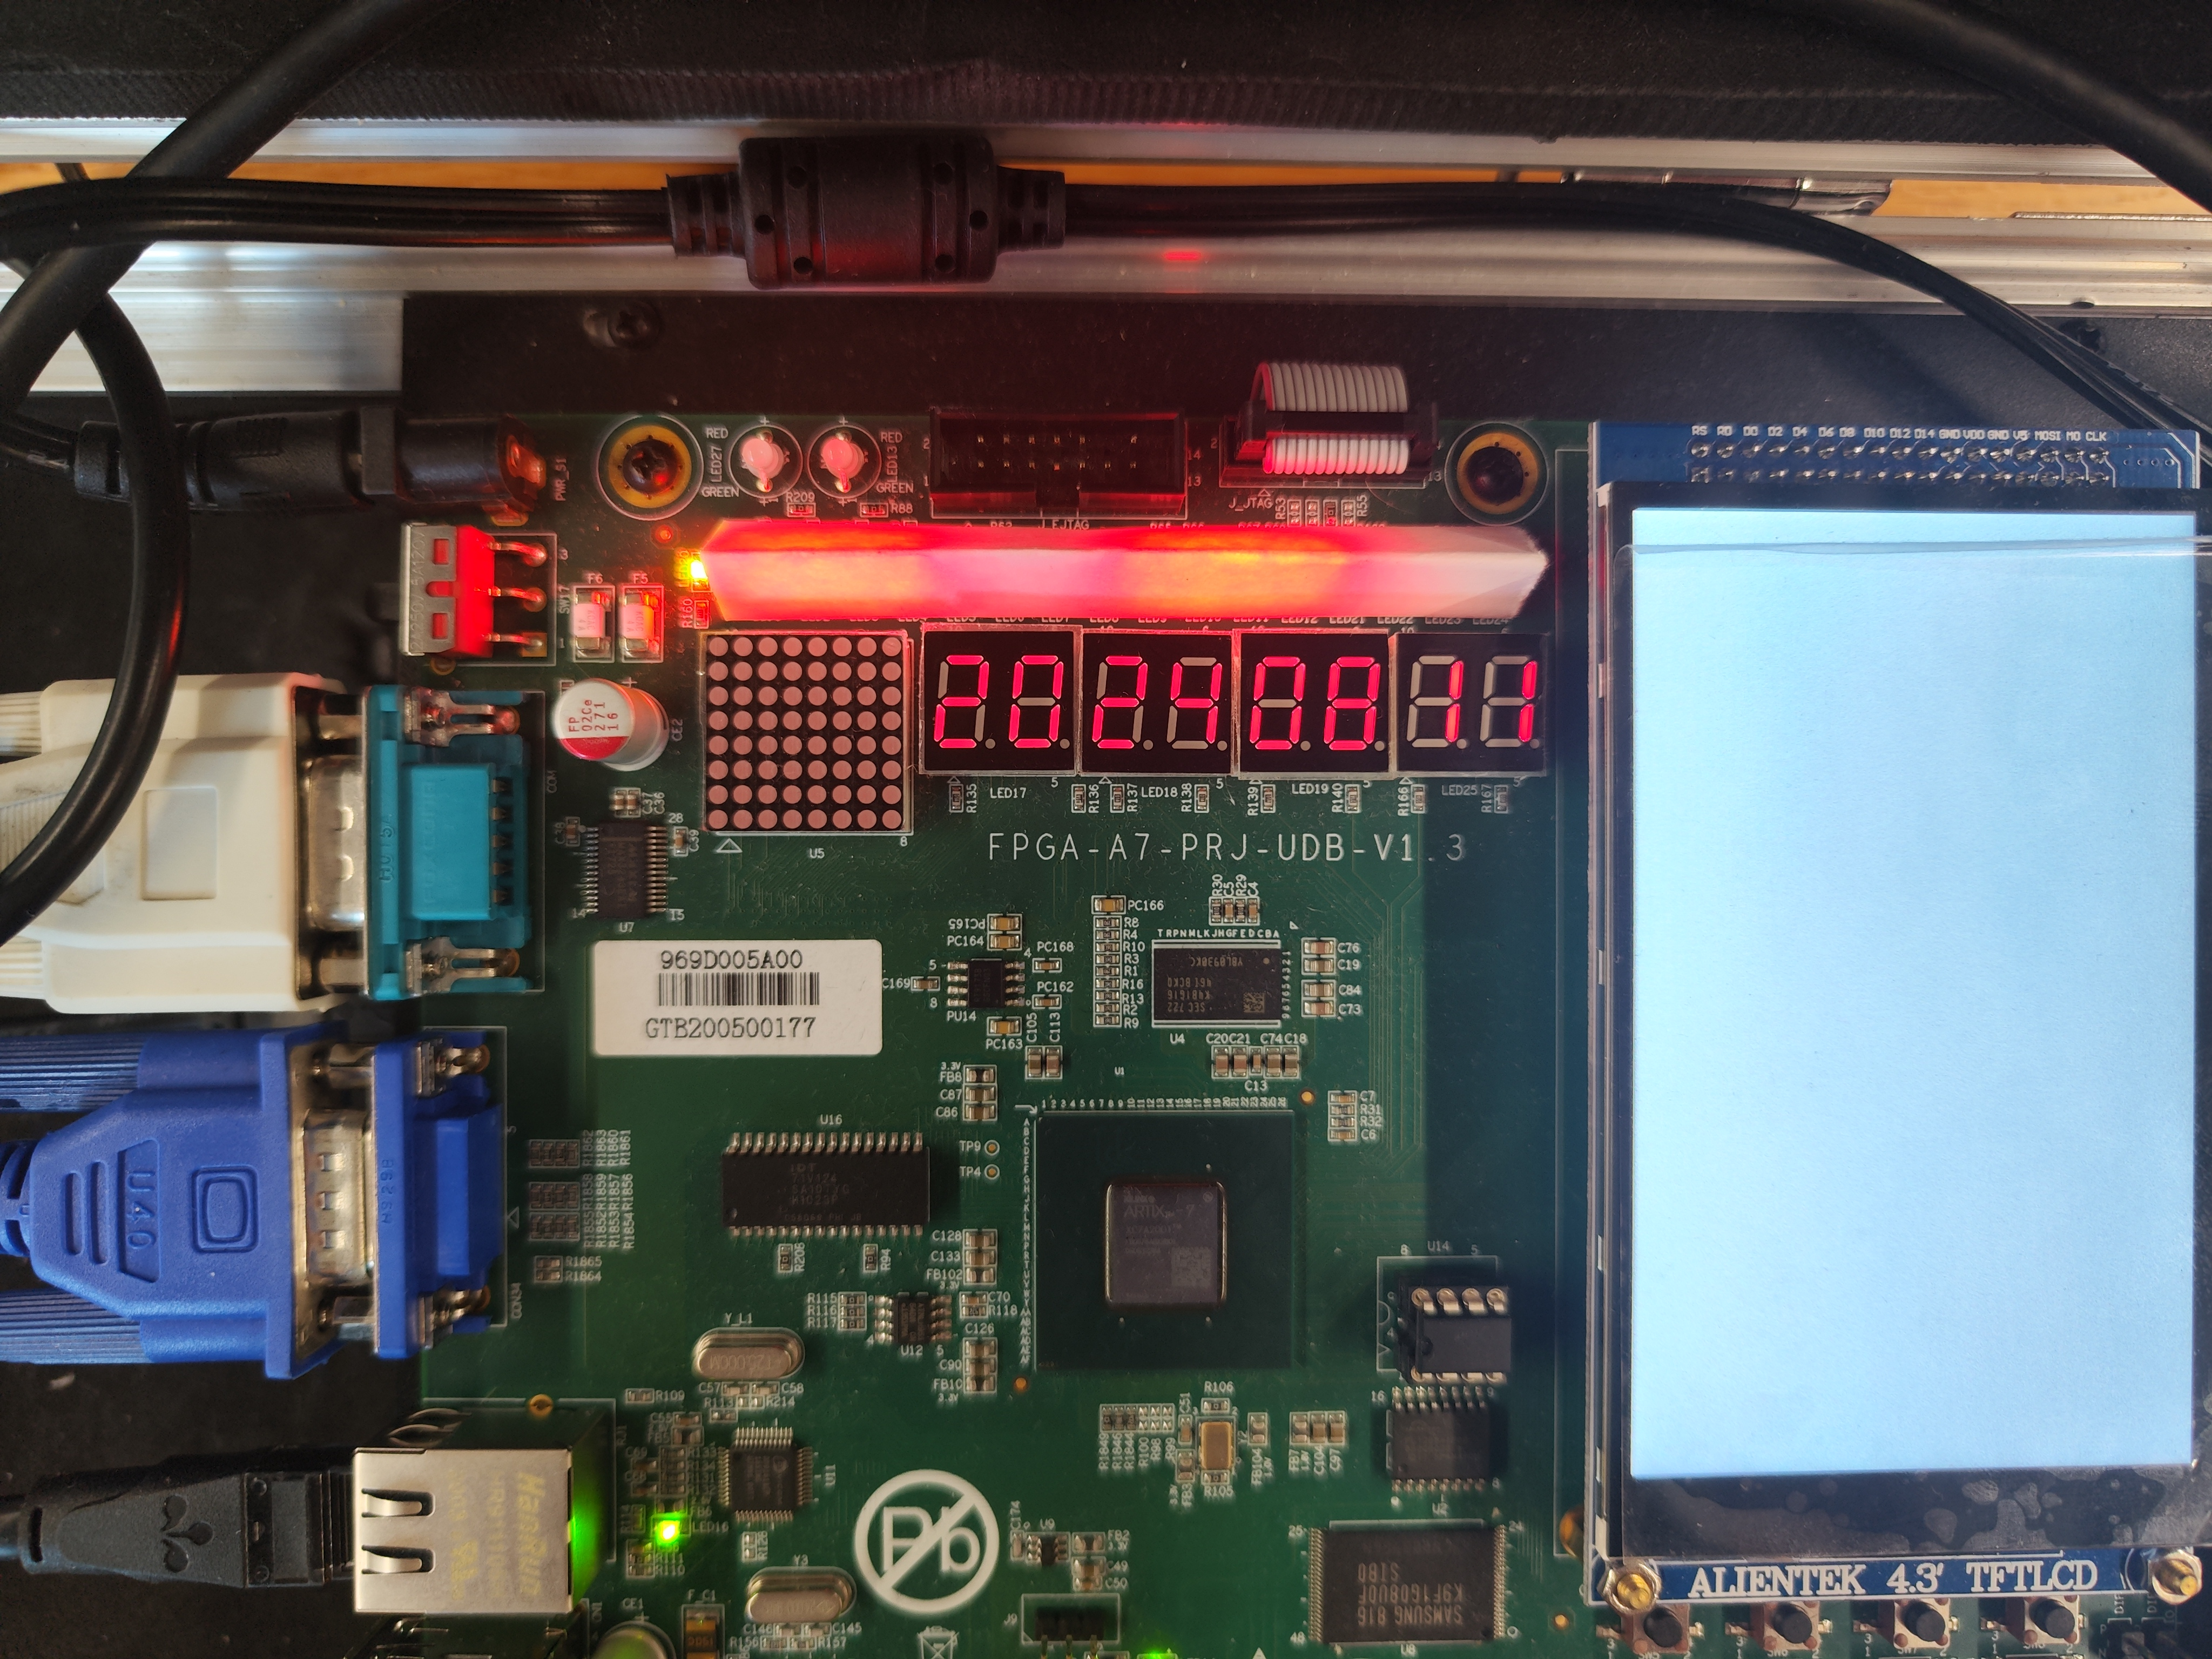
\includegraphics[width=0.5\linewidth]{./imgs/uboot_date.jpg}
    \caption{七段数码管日期显示以及LED灯对应特定位亮(为拍摄效果,使用纸遮挡LED)}
\end{figure}
参照chiplab手册,使用其提供的programmer\_by\_uart工具,将uboot烧录到SPI Flash中,以实现复位后自动进入uboot。然后,在uboot中设置ip,使用tftp传输Linux内核镜像到内存中。最后执行boot命令,启动Linux系统。
\newpage
\subsection{Linux}
本项目以龙芯仓库的la32r-Linux内核为基础,对其进行了修改以适配本项目的硬件平台。以发行版的rootfs为蓝本,在文件系统中新增了2048小游戏等应用程序,并使用busybox提供的用户命令行工具。\par
经测试,iFuProcessor可以稳定启动Linux内核,运行用户程序,驱动LCD等外设。\par

\begin{figure}[htbp]
    \centering
    \begin{minipage}[b]{0.45\textwidth}
      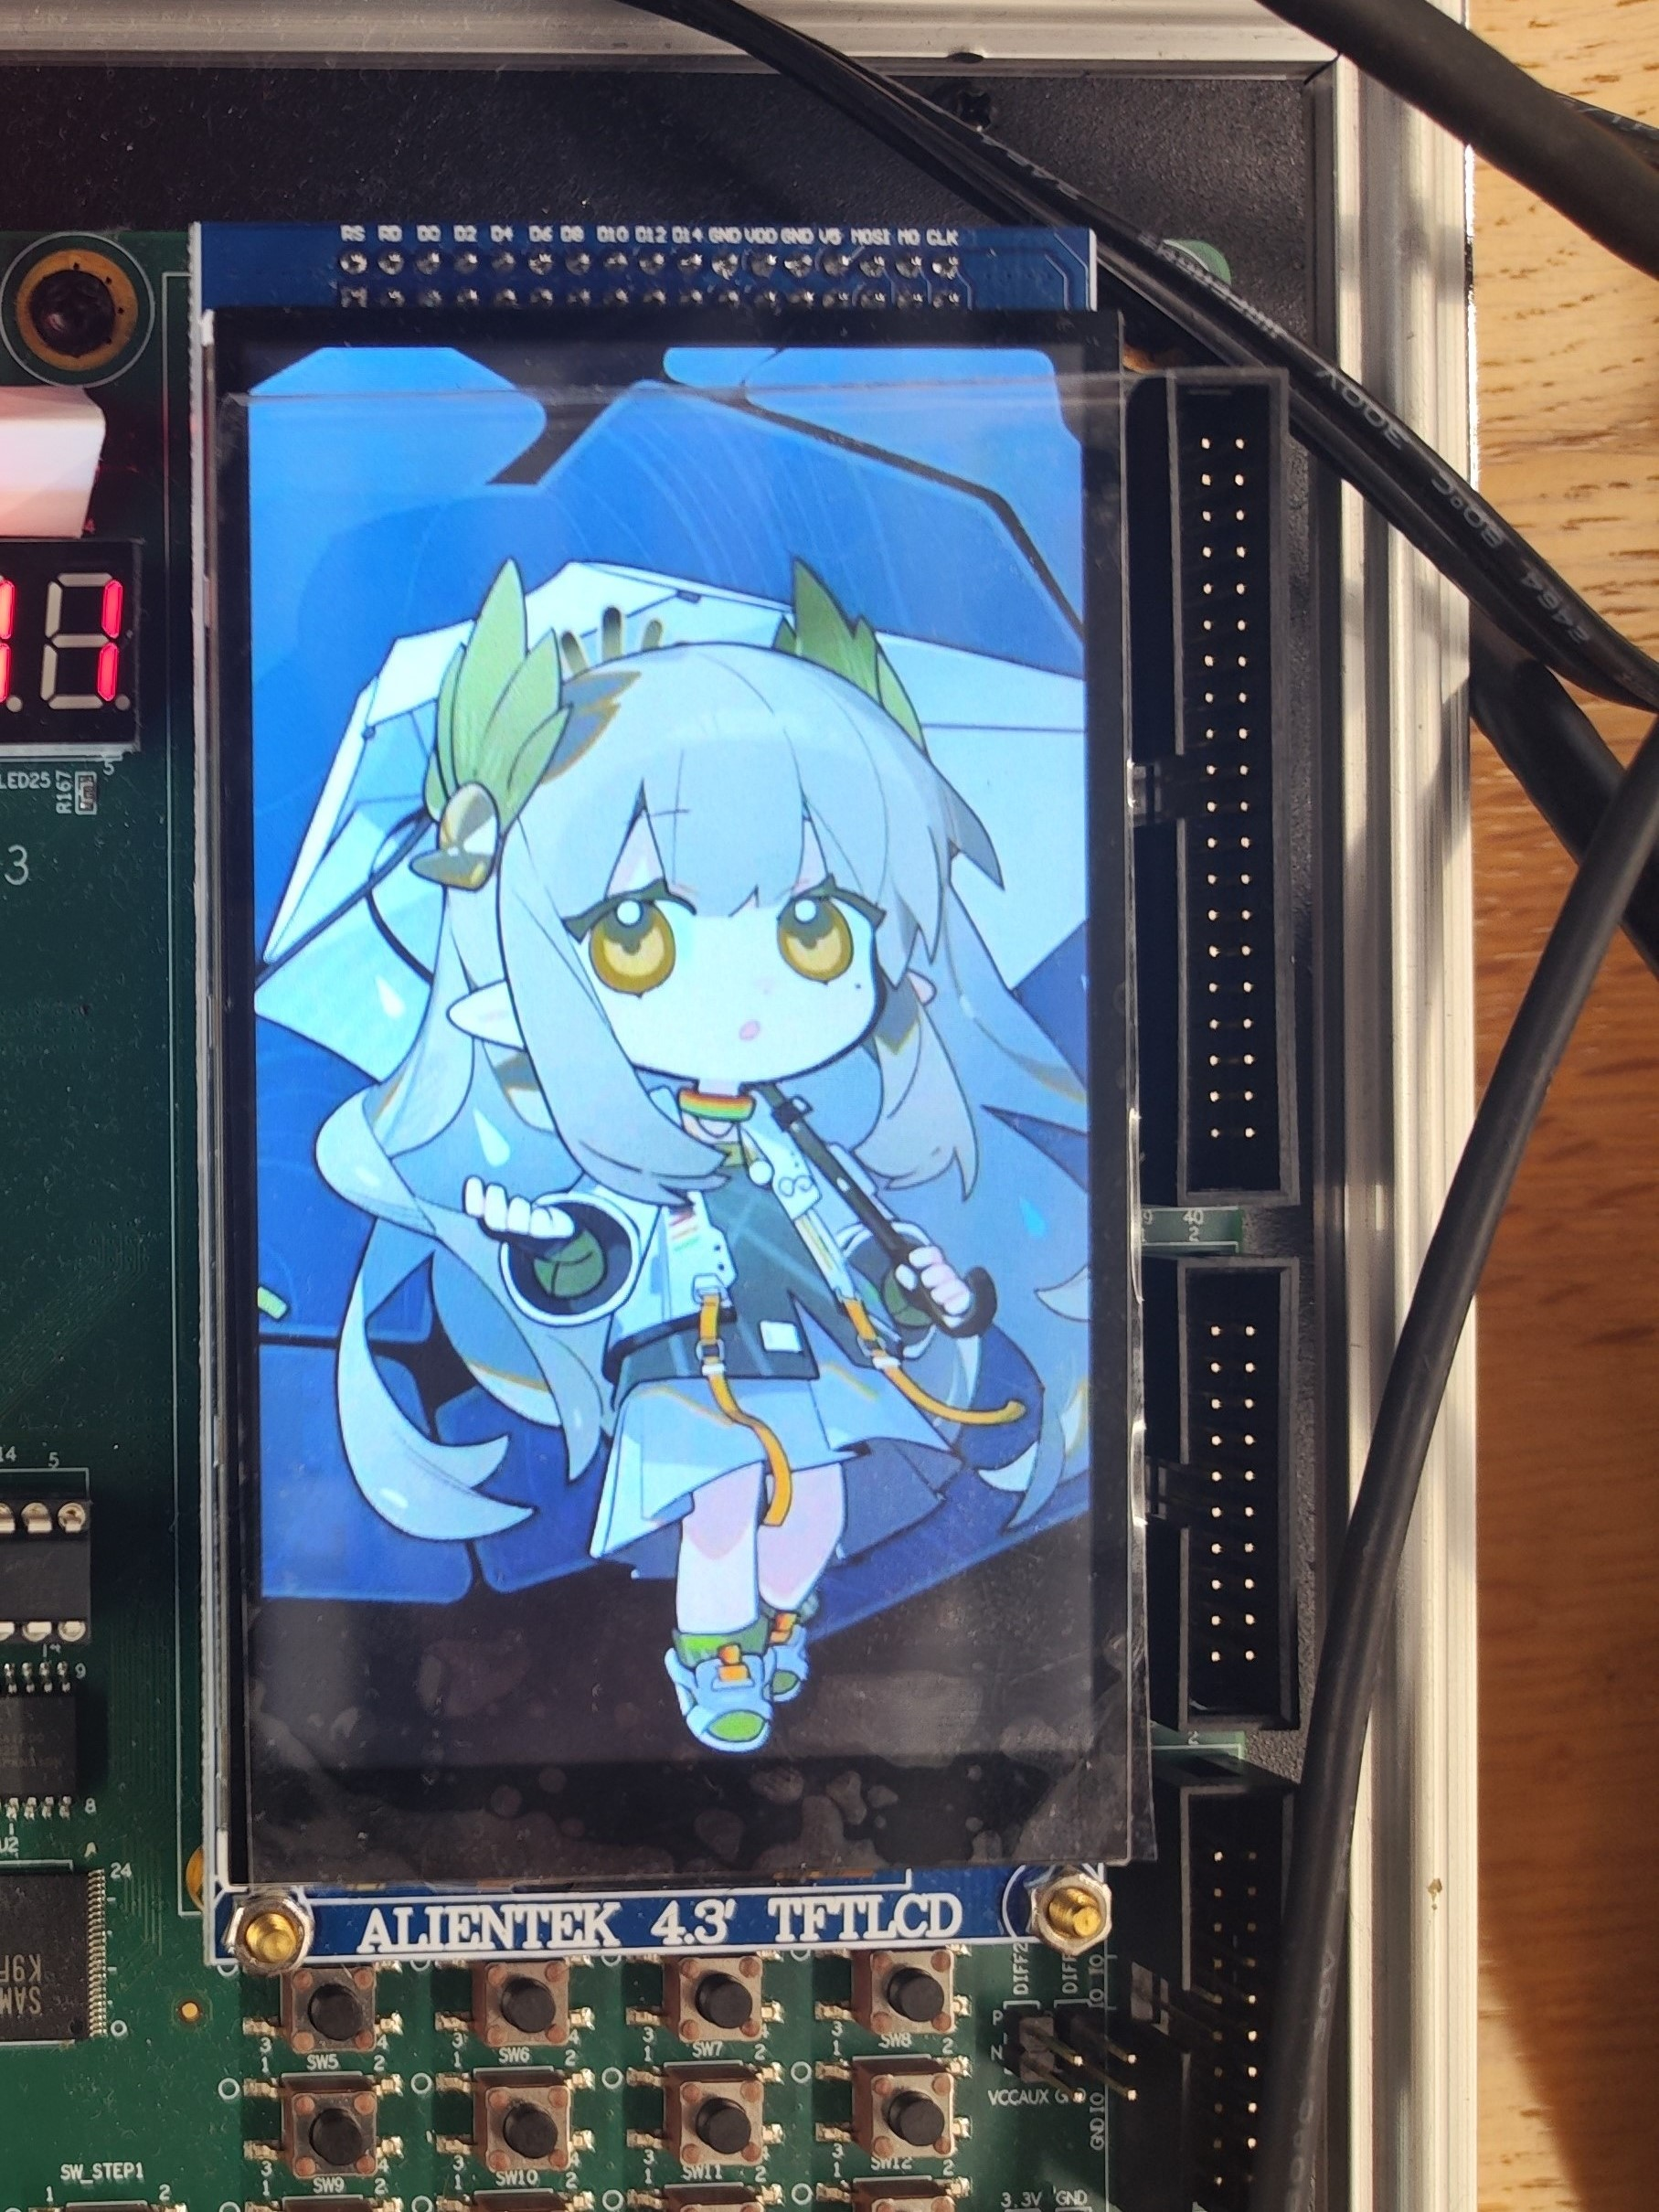
\includegraphics[width=\textwidth]{./imgs/Lcd_show.jpg}
      \caption{Linux驱动LCD外设}
    \end{minipage}
    \hfill 
    \begin{minipage}[b]{0.45\textwidth}
      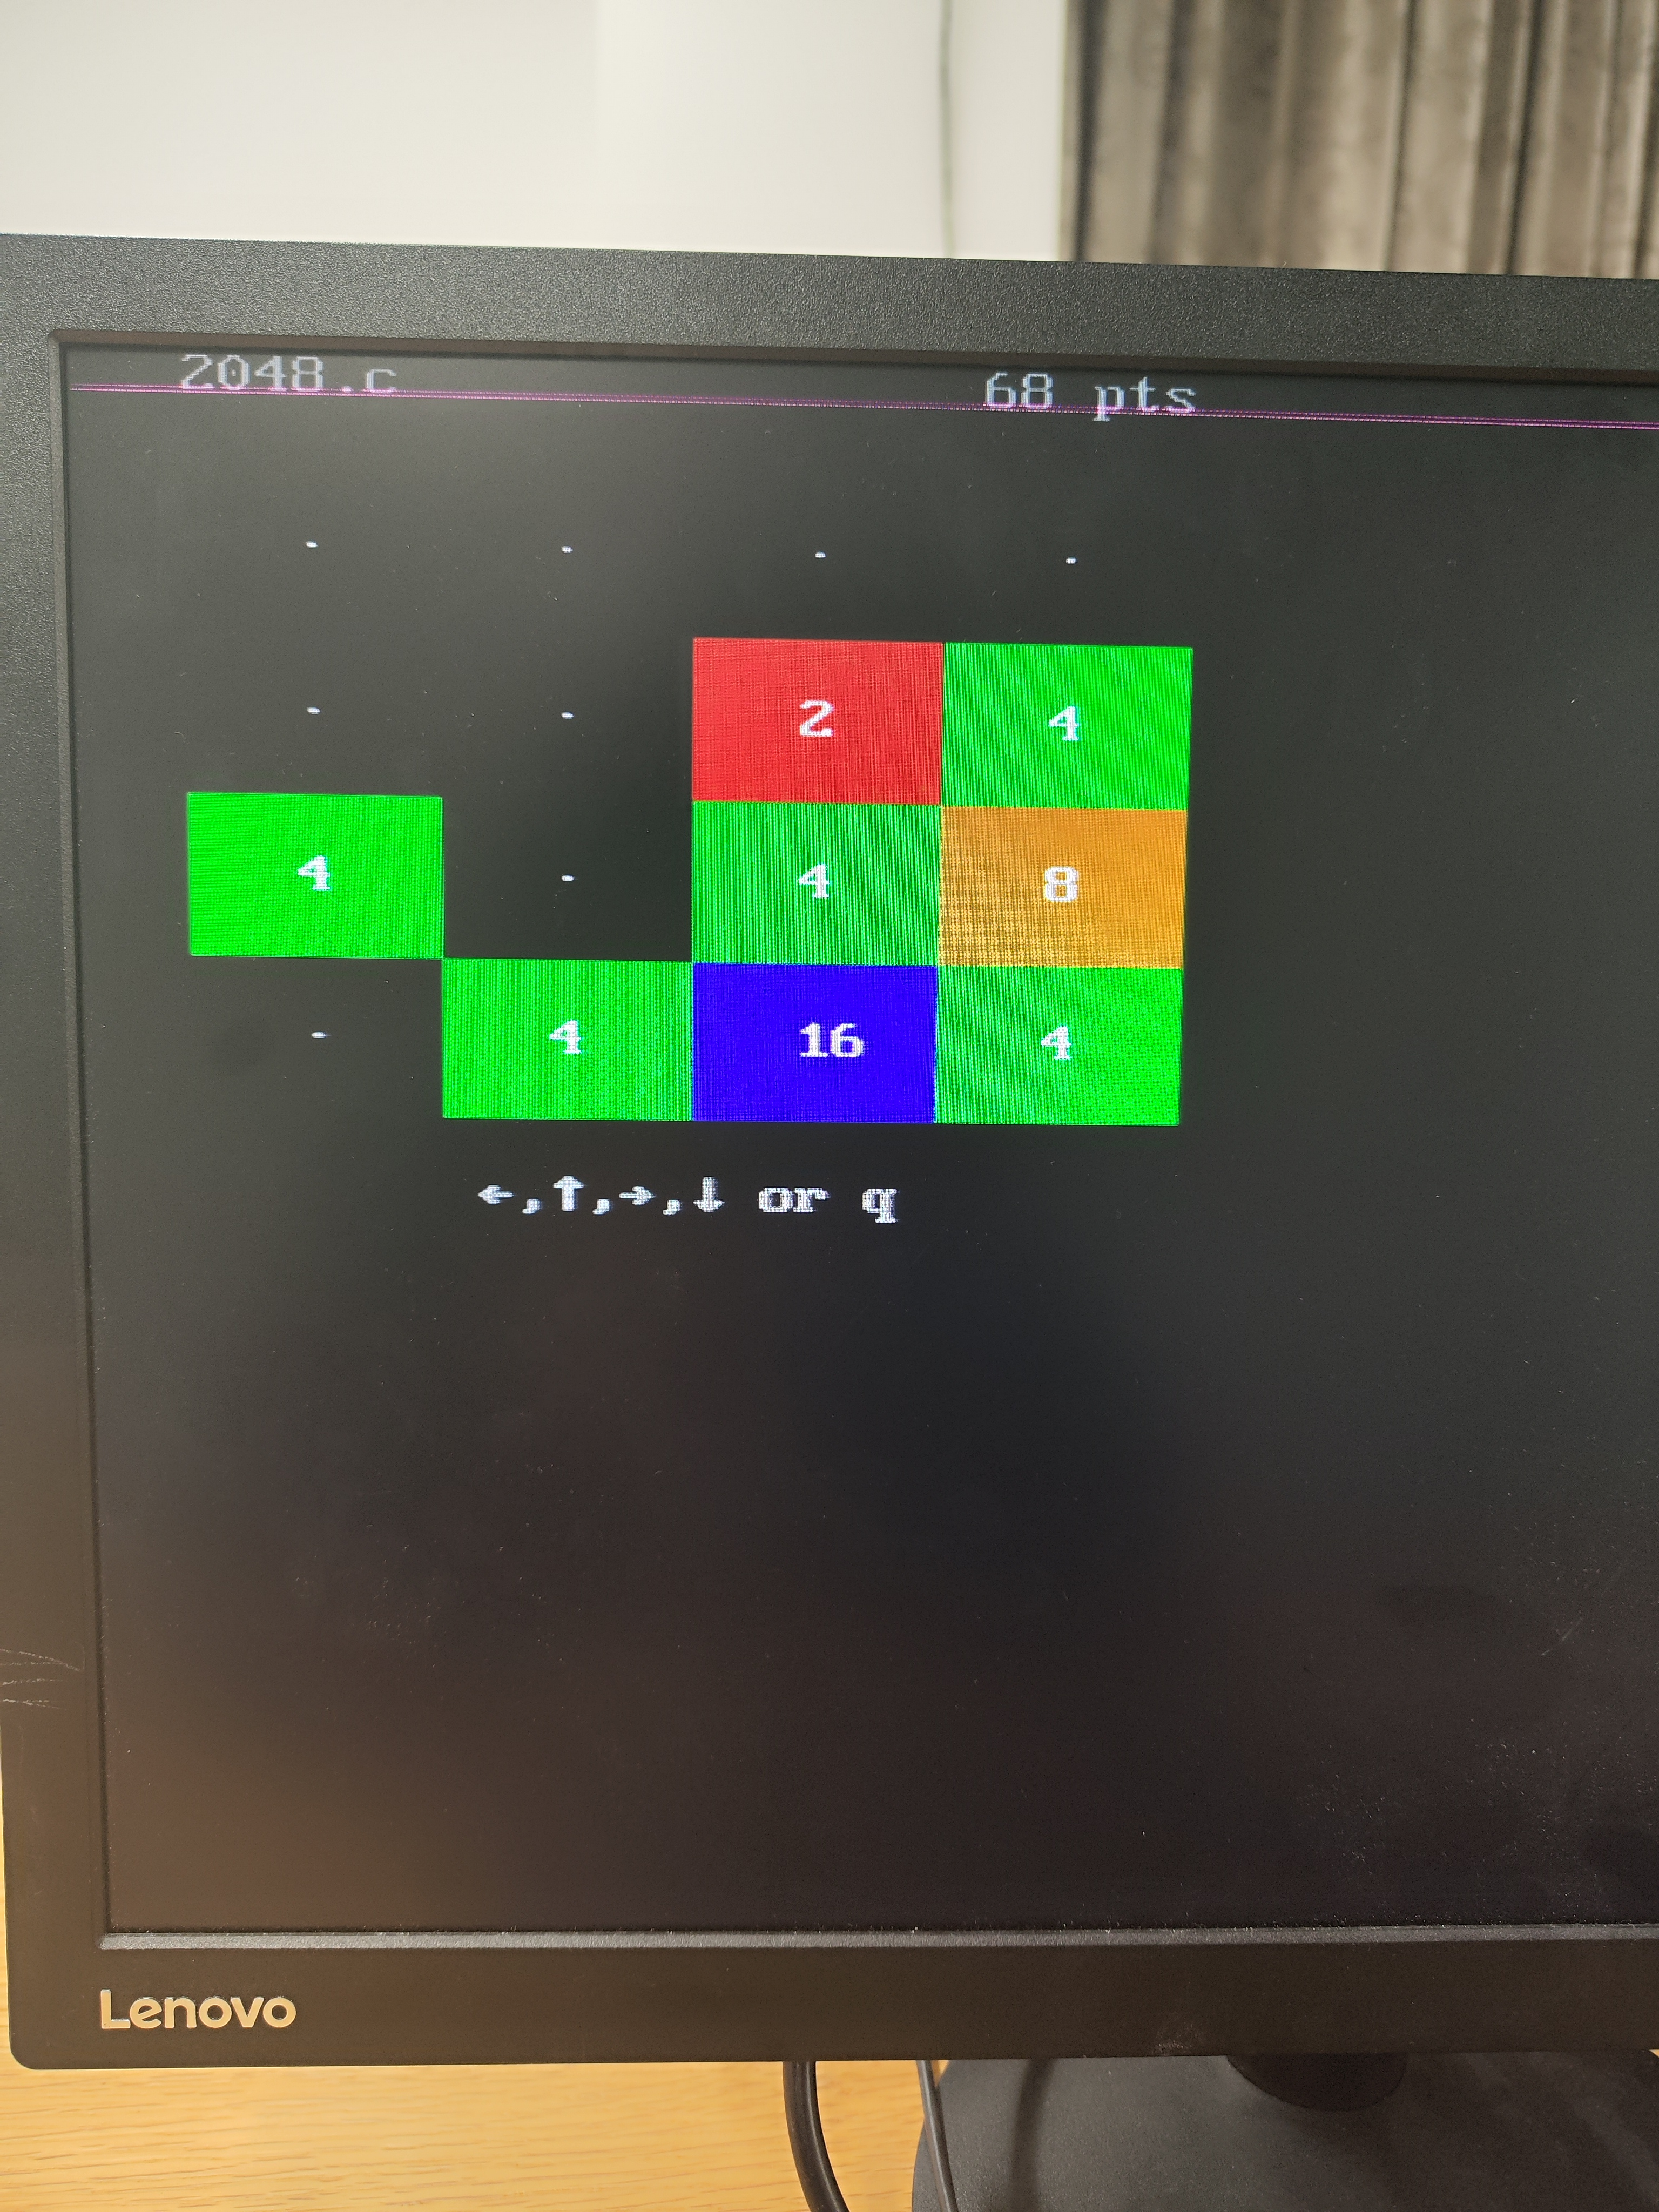
\includegraphics[width=\textwidth]{./imgs/2048.jpg}
      \caption{2048小游戏}
    \end{minipage}
  \end{figure}

\section{参考资料}
在本项目的设计和开发中,参考和借鉴了包括但不限于下列书籍、资料、网站和开源项目:
\begin{itemize}
    \item Chisel 文档:\url{https://www.chisel-lang.org/docs}
    \item The Berkeley Out-of-Order Machine (BOOM)
        \begin{itemize}
            \item 网页:\url{https://boom-core.org/}
            \item 文档:\url{https://docs.boom-core.org/en/latest/}
            \item 仓库:\url{https://github.com/riscv-boom/riscv-boom}
        \end{itemize}
    \item Rocket Chip
        \begin{itemize}
            \item 仓库:\url{https://github.com/chipsalliance/rocket-chip}
        \end{itemize}
    \item 香山处理器
        \begin{itemize}
            \item 文档:\url{https://xiangshan-doc.readthedocs.io/zh-cn/latest/arch/}
            \item 仓库:\url{https://github.com/OpenXiangShan/XiangShan}
        \end{itemize}
    \item NutShell
        \begin{itemize}
            \item 文档:\url{https://oscpu.github.io/NutShell-doc/}
            \item 仓库:\url{https://github.com/OSCPU/NutShell}
        \end{itemize}
    \item Ma-River
        \begin{itemize}
            \item 设计报告:\url{https://github.com/HIT-MaRiver-mips/report-mariver}
            \item 仓库:\url{https://github.com/HIT-MaRiver-mips/cpucore-mariver}
        \end{itemize}
    \item chiplab
        \begin{itemize}
            \item 文档:\url{https://chiplab.readthedocs.io/zh/latest/}
            \item 仓库:\url{https://gitee.com/loongson-edu/chiplab}
        \end{itemize}
    \item FDU1.1-NSCSCC
        \begin{itemize}
            \item 仓库:\url{https://github.com/NSCSCC-2020-Fudan/FDU1.1-NSCSCC/tree/master}
        \end{itemize}
    \item NOP-Processor
        \begin{itemize}
            \item 仓库:\url{https://github.com/NOP-Processor}
        \end{itemize}
    \item 姚永斌.超标量处理器设计[M].清华大学出版社:201404.
    \item 汪文祥,邢金璋.CPU设计实战[M].机械工业出版社:202101.
    \item John L. Hennessy,David A. Patterson.计算机体系结构:量化研究方法[M].人民邮电出版社:202210.
\end{itemize}

\end{document}
